\documentclass[twocolumn,showpacs,preprintnumbers,amsmath,amssymb,pra,aps,superscriptaddress]{revtex4-1}

\usepackage{graphicx}
\usepackage{amsmath}
\usepackage{siunitx}
\usepackage{hyperref}

\begin{document}

\title{Direct Entropy Measurement in a Mesoscopic Quantum System}
\author{Nikolaus Hartman}
\email{nik.hartman@gmail.com}
\thanks{The raw data and Python code used for the figures and analysis can be found at \url{https://github.com/nikhartman/spin_entropy}}
\affiliation{University of British Columbia, Vanouver, BC, Canada}
\author{Saeed Fallahi}
\affiliation{Purdue University, Lafayette, IN, USA}
\author{Geoffrey C. Gardner}
\affiliation{Purdue University, Lafayette, IN, USA}
\author{Christian Olsen}
\affiliation{University of British Columbia, Vanouver, BC, Canada}
\author{Silvia Folk}
\affiliation{University of British Columbia, Vanouver, BC, Canada}
\author{Mohammad Samani}
\altaffiliation{The Hospital for Sick Children, Toronto, ON, Canada}
\altaffiliation{Fields Institute for Research in Mathematical Sciences, Toronto, ON, Canada}
\affiliation{University of British Columbia, Vanouver, BC, Canada}
\author{Michael Manfra}
\affiliation{Purdue University, Lafayette, IN, USA}
\author{Joshua Folk}
\affiliation{University of British Columbia, Vanouver, BC, Canada}
\date{\today}

\begin{abstract}

Measuring the entropy of an electronic state is a powerful tool for identifying its underlying microscopic character.  Such measurements are typically based on bulk properties, such as heat capacity, that are straightforward to observe in macroscopic samples but exceedingly difficult to access in mesoscopic systems, sometimes consisting of just a few electrons. Taking advantage of a well-known Maxwell relation, we realize a mesoscopic geometry in a GaAs heterostructure in which entropy-to-charge conversion enables an entropy measurement of quantum states down to the single electron level. As a demonstration of the efficacy of this method, the entropy of the first few-electron spin states in a gate-defined GaAs quantum dot are measured. The entropy of a single spin ($k_B \ln{2}$) is measured within 8\% accuracy, as is the entropy arising at the magnetic field-driven singlet-triplet crossing for two electrons.

\end{abstract}

\maketitle

%%%%%%% intro material %%%%%%%%%
The thermodynamic properties of electronic systems can offer important insights into the nature of their ground states, and probe exotic quasiparticles that may emerge due to interactions or non-trivial topology.  Systems that are difficult to clearly identify through standard conductance measurements may be studied more in depth if a thermodynamic measurement can be made. For example, the purported non-Abelian exchange statistics of Moore-Read quasiparticles in the $\nu = \frac{5}{2}$ fractional quantum Hall state, or of Majorana quasiparticles in a topological superconductor, are exceedingly difficult to identify from conductance signatures. However, an entropy measurement could clearly distinguish Abelian from non-Abelian quasiparticles \cite{Cooper2009, Smirnov2015}.  Similarly, the two-channel Kondo state that is believed to arise in carefully tuned GaAs devices has so far been identified through a particular temperature dependence in the device conductance \cite{Potok2007}. A more direct test for the two-channel Kondo state would be a confirmation of its entropy ($\frac{1}{2} k_B \ln{2}$), that should remain down to arbitrarily low temperatures \cite{Alkurtass2016}.

%%% figure 1 %%%
\begin{figure}[!]
        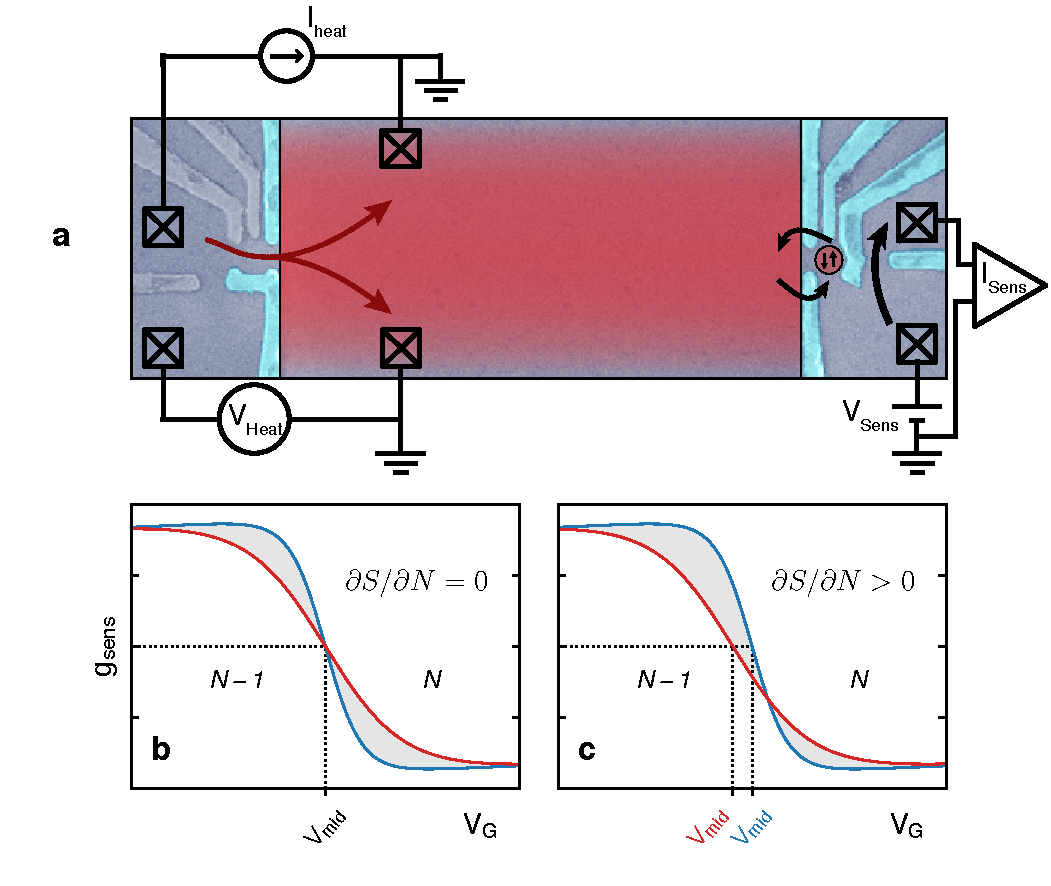
\includegraphics[width=1.0\columnwidth]{../figures/figure_1_no-annotation.pdf}
        \caption{\label{fig:fig1}(a) Scanning electron micrograph of a device similar to the one measured, showing electrostatic gates (blue) used to define a circuit in the 2D electron gas. Grey gates are unused (grounded).  A \SI{1}{\milli\metre}-long channel is formed between the parallel gates running vertically down the image. The channel can be heated by driving current through the constriction on the left.  A 200nm diameter quantum dot is tunnel-coupled to the right side of the channel. Occupation of the dot is monitored by a capacitively-coupled charge sensor. Squares show the locations of ohmic contacts to the 2DEG. (b) Calculated charge sensor signal showing a single transition from $N \rightarrow N+1$ electrons at two temperatures ($T_{Red} > T_{Blue}$). (c) Change in the charge sensor signal with respect to temperature. The asymmetry in peak height arises from the shift in $V_0$ due to the change in entropy, $dS$, between the $N$ and $N+1$ electron states. In the case of $dS=0$, $dg$ is anti-symmetric about $V_0$.}
\end{figure}

While measurements of heat capacity are effective in probing the entropy of macroscopic 3D samples, the heat capacities of single electrons or quasiparticles are much too small to measure directly; even the 2D sheet of quasiparticles in $\nu = \frac{5}{2}$ fractional quantum Hall samples has a heat capacity that vanishes in comparison to the host crystal.  Rather than attempt to resolve such infinitesimal signals, the problem can be avoided by converting a change in entropy to changes in a more easily measured quantity, charge.  Our approach is analogous to the milestone of spin-to-charge conversion, first demonstrated in GaAs quantum dots in 2004, by which undetectably-small magnetic moments of a single spin were transformed into thepresence or absence of an electron charge, which is easily detected4 \cite{Elzerman2004, Ono2004}.

In order to accomplish this entropy to charge conversion, we make use of the Maxwell relation
%
\begin{align}
\label{eqn:max}
        \left(\frac{\partial \mu}{\partial T}\right)_{p,N} &= -\left(\frac{\partial S}{\partial N}\right)_{p,T}
\end{align}
%
that connects changes in entropy, $S$, (as well as particle number $N$ and temperature $T$) to changes in the chemical potential, $\mu$, a quantity that is simple to measure and control. The fixed pressure condition is met by working well below the Fermi temperature, $T_F \sim$\SI{5}{\kelvin}, where the pressure is simply the degeneracy pressure \cite{Landau1969}. Refs.~\onlinecite{Cooper2009} and ~\onlinecite{Ben-Shach2013} propose schemes to measure the entropy derivative, $\frac{\partial S}{\partial N}$, of the $\nu = \frac{5}{2}$ state via this Maxwell relation, detecting changes in the quasiparticle chemical potential with temperature.  Our work builds on these ideas to measure the entropy of the few-electron ground states of a quantum dot. Unlike the $\nu = \frac{5}{2}$ quasiparticles described in the theoretical work, the few-electron quantum dot states studied here have an entropy that is well-understood from the spin degree of freedom \cite{Tarucha1996, Ciorga2000, Duncan2000, Lindemann2002, Potok2003, Hofmann2016}. This work demonstrates a direct thermodyanmic measurement on a simple few-particle system; the method can be easily extended as a probe into the nature of more exotic systems ,such as topologically non-trivial Majorana and other non-Abelian states.

The mesoscopic circuit shown in Fig.~\ref{fig:fig1}a realizes an electron reservoir (central region) in thermal equilibrium with a few-electron quantum dot coupled to its right side, where tunneling between the two is measured using a charge sensing QPC capacitively coupled to the dot \cite{Staring2007, Frolov2009, Thierschmann2015}. The number of electrons on the dot can be tuned using the gate voltage, $V_G$. An electron is added to an $N$ electron dot when the chemical potential to add an electron, $\mu_{N+1}$ (proportional to $V_G$), drops below the Fermi level of the reservoir, $E_F$.  Figure 1b illustrates a such a transition, as measured by the charge sensor conductance, as a function of $V_G$. The gate voltage corresponding to midpoint of the transition, $V_0$, marks the chemical potential where the probabilties of finding $N$ or $N+1$ electrons on the dot are equal. This transition is thermally broadened by the reservoir temperature $T_{res}$. Additionally, an entropy change from the $N$ to $N+1$ ground states of the dot can shift the midpoint of the transition, $V_0$, by changing the chemical potential on the dot as in Eq.~\ref{eqn:max}.  Detecting the shift in $V_0$ with respect to temperature (${\propto}\frac{\partial \mu}{\partial T}$), amounts to a measurement of the entropy difference $dS$ between the $N$ to $N+1$ ground states ($dN=1$).  In practice, the shift in $V_0$ is measured by oscillating $T_{res}$ and monitoring changes in $g_{sens}$ with a lockin amplifier.  Consider the charge transitions in Fig.~\ref{fig:fig1}b, if the warmer transition is not only broadened but shifted ($dS\neq0$), the change in $g_{sens}$ is asymmetric as shown in Fig.~\ref{fig:fig1}c; if the warmer transition is broadened but not shifted with respect to the cooler one ($dS=0$), the lineshape is anti-symmetric.

An explanation based on detailed balance is helpful in understanding how a shift in $\mu_{N+1}$ (relative to $E_F$) relates to entropy. Tunneling between the dot and reservoir is possible when the chemical potential to add an electron, $\mu_{N+1}$, is within ${\sim}3.5 k_B T$ of Fermi level of the reservoir. Away from that window, tunneling is suppressed due to a lack of available states in the reservoir. To illustrate how the tunnel rates, $\Gamma_{in}=\Gamma_{N\rightarrow N+1}$ and $\Gamma_{out}=\Gamma_{N+1\rightarrow N}$ depend on degeneracy, consider the filling of the first electron state. The 1-electron ground state has a degeneracy of 2 due to a single, unpaired spin-$\frac{1}{2}$; electrons tunneling into this state have both spin-up and -down states available. Conversely, an electron tunneling off of the dot must tunnel into a state with its same spin, that is, only half of the reservoir states are available to it. As a result, $\Gamma_{in} = 2\Gamma_{out}$ when $\mu_{N+1}=E_F$. Extending this logic to a general case gives the same results as derived from detailed balance \cite{Gustavsson2009}, 
%
\begin{align}
	\Gamma_{in} &=  g_{N+1} \Gamma f(E_F - \mu_{N+1}) \label{eqn:gin}\\
	\Gamma_{out} &= g_{N} \Gamma [1 - f(E_F - \mu_{N+1})] \label{eqn:gout}
\end{align}
%
where $\Gamma$ is a coupling constant and $g_{N/N+1}$ are the degeneracies of the $N$ and $N+1$ electron states.. The midpoint of the transition between the $N$ and $N+1$ electon states, measured by the charge sensor, occurs when the $\Gamma_{in} = \Gamma_{out}$. It is clear from Eqs.~\ref{eqn:gin} and \ref{eqn:gout}, that in the case $g_{N}=g_{N+1}$, $\Gamma_{in} = \Gamma_{out}$ when $\mu_{N+1} = E_F$. However, if the two occupation states differ in their degeneracy, the midpoint of the transition shifts away from $\mu_{N+1}=E_F$. Thermal broadening of the Fermi functions in Eqs.~\ref{eqn:gin} and \ref{eqn:gout} means that the chemical potential at which $\Gamma_{in} = \Gamma_{out}$ depends on $T$ as well as $g_{N/N+1}$. By measuring $dV_0$ ($d_\mu$) as a function of $dT$, the ratio $g_{N+1}/g_{N}$ can be determined, which is related to $dS$ through the Boltzmann entropy. The relationship between degeneracies and tunnel rates was recently explored in a time-resolved measurement \cite{Hofmann2016}.  The thermal technique presented here extends the measurement of entropy (degeneracy) to a wider set of applications, where the tunneling process may not be convenient or even possible to observe directly.

%%% fab/measurement details %%%
The device was built on a AlGaAs/GaAs heterostructure, hosting a 2D electron gas with density and mobility at \SI{300}{\milli\kelvin} (determined on a separate chip) of \SI{2.42e11}{\per\square\centi\metre} and \SI[per-mode=symbol]{2.56e6}{\square\centi\metre\per\volt\per\second}.   Mesas and NiAuGe ohmic contacts to the 2DEG were defined by standard photolithography techniques, then \SI{10}{\nano\metre} of $\mathrm{HfO_2}$ was deposited via atomic layer deposition to improve the gating stability to the device. Electron beam lithography followed by evaporation of \SI{20}{\nano\metre} of Ti/Au defined the fine gate structures, including the \SI{200}{\nano\metre} diameter quantum dots. The measurement was carried out in an dilution refrigerator with a base temperature of \SI{14}{\milli\kelvin}.

%%%%%%%%%%  current edits end here  %%%%%%%%%%%%%

%%% figure 2 %%%
\begin{figure}[!]
        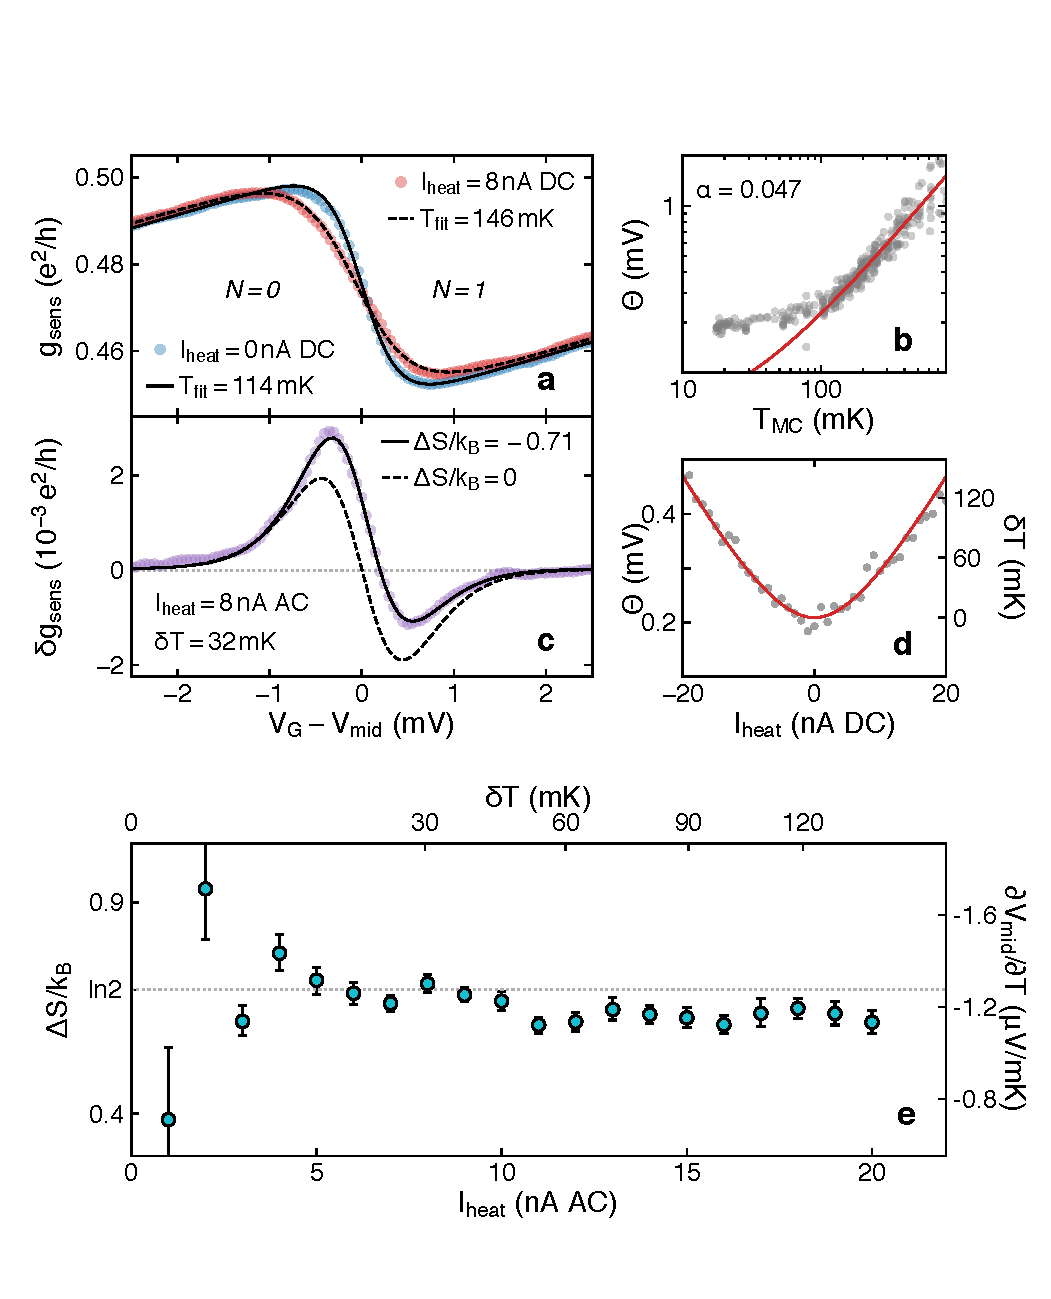
\includegraphics[width=1.0\columnwidth]{../figures/figure_2.pdf}
        \caption{\label{fig:fig2}(a) Charge sensor data for $N=0 \rightarrow 1$ at 100 and 160mK. Temperature is set by DC current through the QPC heater. (b) Derivative of the charge sensor signal with $dT \sim 60mK$. Fits to $dg$ are shown with $\delta$ as a free parameter (solid) and $\delta=0$ (dashed) (c) Transition width, $\Theta$, as a fucntion of mixing chamber temperature. The highlighted, linear region is where all the data discussed were measured. Fitting a straight line to this data, the lever arm $\alpha$ is calculated. (d) $\Theta$ as a function of DC current through the QPC heater. The linear fit is used to convert between $I_{heat}$ and $dT$, with $R_{QPC}$ fixed at 20$k\Omega$ (e) Change in entropy as a function of AC current through the QPC heater. Top axis shows corresponding $dT$. (f) Raw data from which $dS / k_B$ in (c), and the line cut in (b) were extracted.}
\end{figure}

To make a  measurement of the quantum dot entropy, the right dot was coupled to the reservoir on the source (left) side, with the drain (right) side of the dot closed. The charge sensing QPC  was tuned to a conductance of ${\sim}e^2/h$. A small DC voltage bias was applied and the measured current was used to calculate the sensor conductance.  Assuming the source barrier is in the limit where single electron transitions ($\Gamma_{In/Out}$) are only broadened by the temperature of the reservoir (discussed further in Fig. \ref{fig:fig2}c, the charge sensor conductance takes the form,
%
\begin{align}
\label{eqn:g}
        g_{sens}(V,\Theta) &= G_0 \tanh\left(\frac{V-V_0(\Theta)}{2\Theta}\right)  \\
                        &\quad + G_1\left[V-V_0(\Theta)\right] + G_2 \nonumber
\end{align}
%
where $\Theta = \frac{k_B T}{\alpha e}$, $\alpha$ is the lever arm for the quantum dot plunger gate, and $G_1$ is determined by the cross capacitance between the sensor gates and the plunger gate.

The temperature of the electron reservoir was varied by applying an AC current through the heating QPC on the left side of the channel. Fluctuations in $g_{sens}$ were measured at $2f_{Heat}$ using a lock-in amplifier; the temperature of the reservoir goes as $dT^2 \sim P^{AC}_{Heat} \sim \sin^2(2\omega t)$. Taking a derivative of Eq. \ref{eqn:g} with respect to temperature gives the change in conductance, $dg_{sens}$, as measured by the lock-in amplifier,
%
\begin{align}
\label{eqn:dg}
        dg_{sens}(V, \Theta) &\propto \left[ \frac{V-V_0(\Theta)}{2\Theta} + \delta \right]\times \\
        				      &\quad\cosh^{-2}\left(\frac{V-V_0(\Theta)}{2\Theta}\right) \nonumber
\end{align}
%
where $\delta=\frac{\partial V_0}{\partial \Theta}$. By using the lever arm to convert $V_0$ to chemical potential $\mu$, and recalling Eq. \ref{eqn:max}, the parameter $\delta$ can be related to the change in entropy,
%
\begin{align}
\label{eqn:delta}
        \delta &= \frac{\partial V_0}{\partial \Theta} = 
        \frac{1}{k_B} \frac{\partial \mu}{\partial T} = 
        -\frac{1}{k_B} \frac{\partial S}{\partial N}
\end{align}
%

The entropy measurement requires no further calibration to extract the desired results from the $dg$ fits. However, it is necessary to ensure that the range of temperatures and energies fit the analysis. To begin, the dot is depleted by tuning the plunger gate and identifying the empty dot using the charge sensor. Typical charge sensor curves for the $N=0 \rightarrow 1$ transision are shown in Fig. \ref{fig:fig2}. The width of the charge sensor signal, determined by fitting Eq. \ref{eqn:g}, is measured as a function of the mixing chamber temperature in Fig. \ref{fig:fig2}c). At a sufficiently high temperature, $T_{electron}=T_{MC}$, and the transition width is determined only by $T_{MC}$ (highlighted region in Fig. \ref{fig:fig2}c). A line fit to $\Theta = \frac{k_B T_{MC}}{\alpha e}$ is used to determine $\alpha$. The remainder of the measurements are performed in the linear region of Fig. \ref{fig:fig2}c at $T_{MC} = 100mK$, where Eqs. \ref{eqn:g} and \ref{eqn:dg} are valid. Fig. \ref{fig:fig2}d shows the calibration of $dT$ as a function of DC current through the QPC heater ($P_{Heat} = I^2_{Heat} R_{QPC}$). Using $\alpha$ to convert from $\Theta$ to $T_{electron}$, the linear fit Fig. \ref{fig:fig2}d gives the the conversion from $I_{Heat}$ to $dT$. To avoid thermally accessing excited states of the dot it must be true that $k_B dT \ll \Delta$ where $\Delta$ is the level spacing between the ground and first excited states; which holds for all transitions investigated.

Data in Fig. \ref{fig:fig2}b show the change in quantum dot entropy determined directly from the lock-in signal, $dg_{sens}$. Fits to Eq. \ref{eqn:dg} are shown for $\delta=0$ (dashed) and a best fit to $\delta$ (solid). It is clear from these fits, $\delta$ is necessary to properly fit the asymmetry in peak height, with the best fit being $\delta \approx \ln{2}$. This is easily understood from the Boltzmann entropy. For an N-electron macrostate on the quantum dot, entropy is given by,
%
\begin{align}
\label{eqn:S}
        S &= k_B \ln{\Omega}
\end{align}
%
where $\Omega$ is the number of microstates available. The number of microstates is equal to the spin degeneracy of the ground state. For the 0-1 transition, this gives $dS =  k_B\ln{2} - k_B \ln{1} = k_B\ln{2}$.

Because $\delta$ is a fit parameter independent of $dT$, it is possible to extract the same $\delta$ value for a range of $dT$ ($I^{AC}_{Heat}$). Fig. \ref{fig:fig2}e shows that $dS$, as determined from $dg_{sens}$ fits, remains constant over a range of $dT$. Looking at the vertical scale on the right side of Fig. \ref{fig:fig2}e, the same shift in chemical potential on the dot is given in units of gate voltage shift per unit temperature change. This illustrates why the lock-in measurement was utilized; device stability and small signals made it difficult for the entropy to be determined directly from $g_{sens}$ using DC heating.

%%% figure 3 %%%
\begin{figure}
        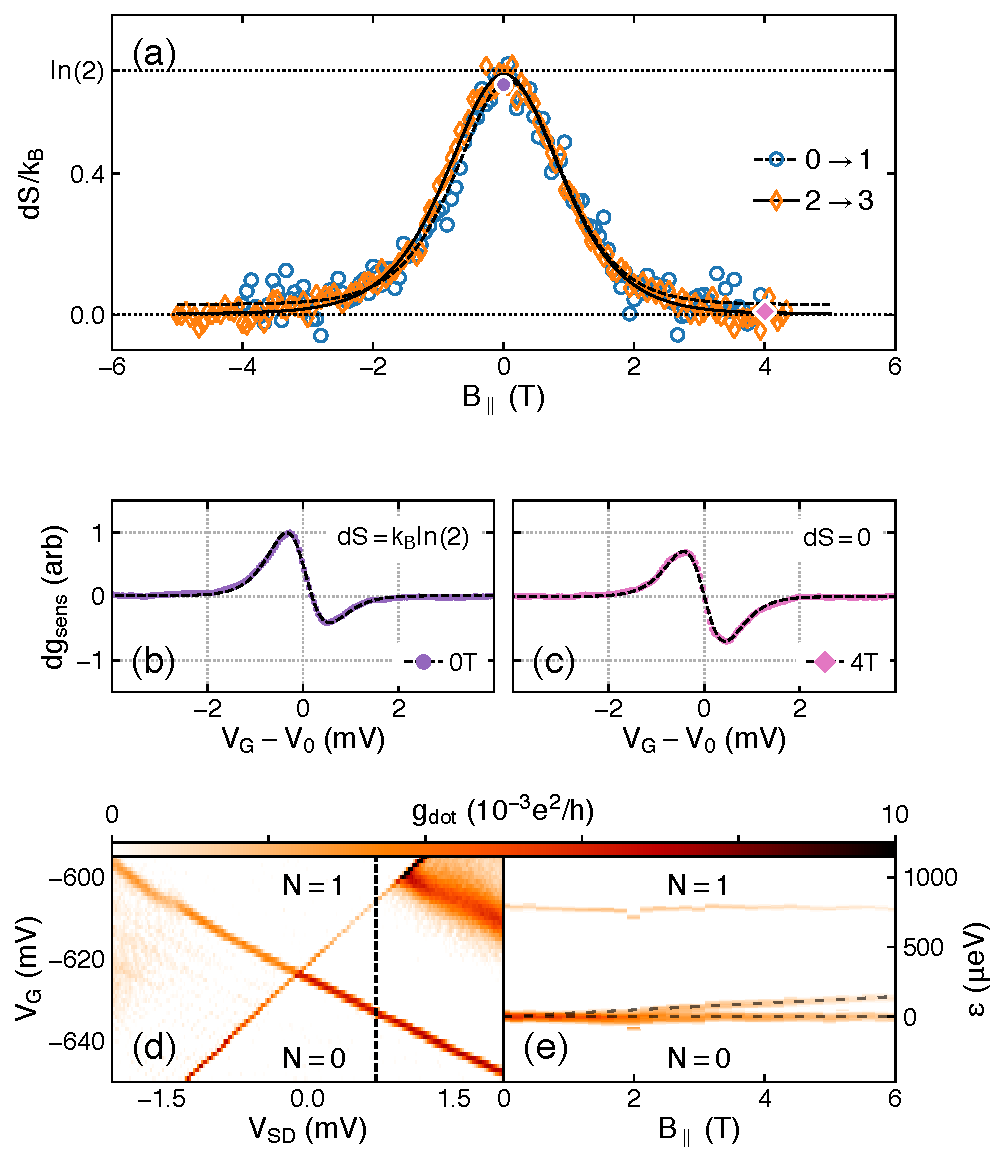
\includegraphics[width=1.0\columnwidth]{../figures/figure_3.pdf}
        \caption{\label{fig:fig3}(a) Transport data through the quantum dot showing the $N=0 \rightarrow 1$ transition. The first excited state, near $V_{SD}$ = \SI{1}{\milli\electronvolt}, is well-above all other energy scales in the measurement. Dashed line shows where data in (b) are taken. (b) Fixed bias transport data ($V_{SD}$ = \SI{700}{\micro\electronvolt}) showing fits to the Zeeman splitting of the ground state energy. (c) Change in entropy, extracted from $dg$ fits, as a function of parallel field. The $N=0 \rightarrow 1$ and $2 \rightarrow 3$ are overlaid here to show the behavior is the same at low parallel field. (d) and (e) show characteristic $dg$ traces from which the data in (c) were extracted.}
\end{figure}

Fig. \ref{fig:fig3}c shows $dS$ as a function of parallel field for the 0-1 (and 2-3) electron transitions. The spin-$\frac{1}{2}$ degeneracy of the 1-electron ground state is lifted as the field increases to \SI{\pm5}{\tesla}.  As the Zeeman splitting, measured directly in Fig. \ref{fig:fig2}b, lifts the spin degeneracy, the entropy of the 1-electron state goes to zero. The 2-3 electron transition behaves similarly at low fields.  The 2-electron ground state is the spin singlet, and the 3-electron ground state is same singlet with an additional unpaired electron, with degeneracy of 2, as in the 1-electron case. Below \SI{5}{\tesla} $g\mu_B B$ remains the largest energy scale, and no 3-electron excited states need be considered.

To understand the behavior of $dS$ as a function of magnetic field, Eq. \ref{eqn:S} can be rewritten as,
%
\begin{align}
\label{eqn:Sp}
        S &= k_B \sum_{i=\pm} p_{i}(B, T) \ln{ p_{i}(B,T) }
\end{align}
%
where $p_{i}(B, T)$ is the probabilty of the system being in the i$^{th}$ microstate at a given field and temperature. The 1 and 3-electron ground states have only a spin-$\frac{1}{2}$ degree of freedom at low field and $p_{i}(B, T)$ can be written as a two-level system,
%
\begin{align}
\label{eqn:p}
        p_{\pm}(B, T) &= \frac{1}{1+ e^{\mp \frac{g\mu_B B}{k_B T}}}
\end{align}
%
where $\pm$ represent the spin up/down states of the unpaired electron.

The dashed and solid lines in Fig \ref{fig:fig3}c show fits to $dS$ using Eqs. \ref{eqn:Sp} and \ref{eqn:p} for the 0-1 and 2-3 electron transitions, respectively. These fits allow for peak height, g-factor, and a vertical offset as free parameters; $T$ is fixed at the mixing chamber temperature. From these fits, $dS=0.92 \ln{2}$ and $g=-0.33$. The peak height, corresponding to $dS(B=0)$, deviates from the expected value because it is convoluted with the vertical offset, caused by the cross-capacitance between plunger and QPC gates. The discrepancy between $g$ and the result in Fig. \ref{fig:fig3}b, can be understood from the change in shape of the quantum dot when tuning between the open and closed drain configurations [citation?].

%%% figure 4 %%%
\begin{figure}
        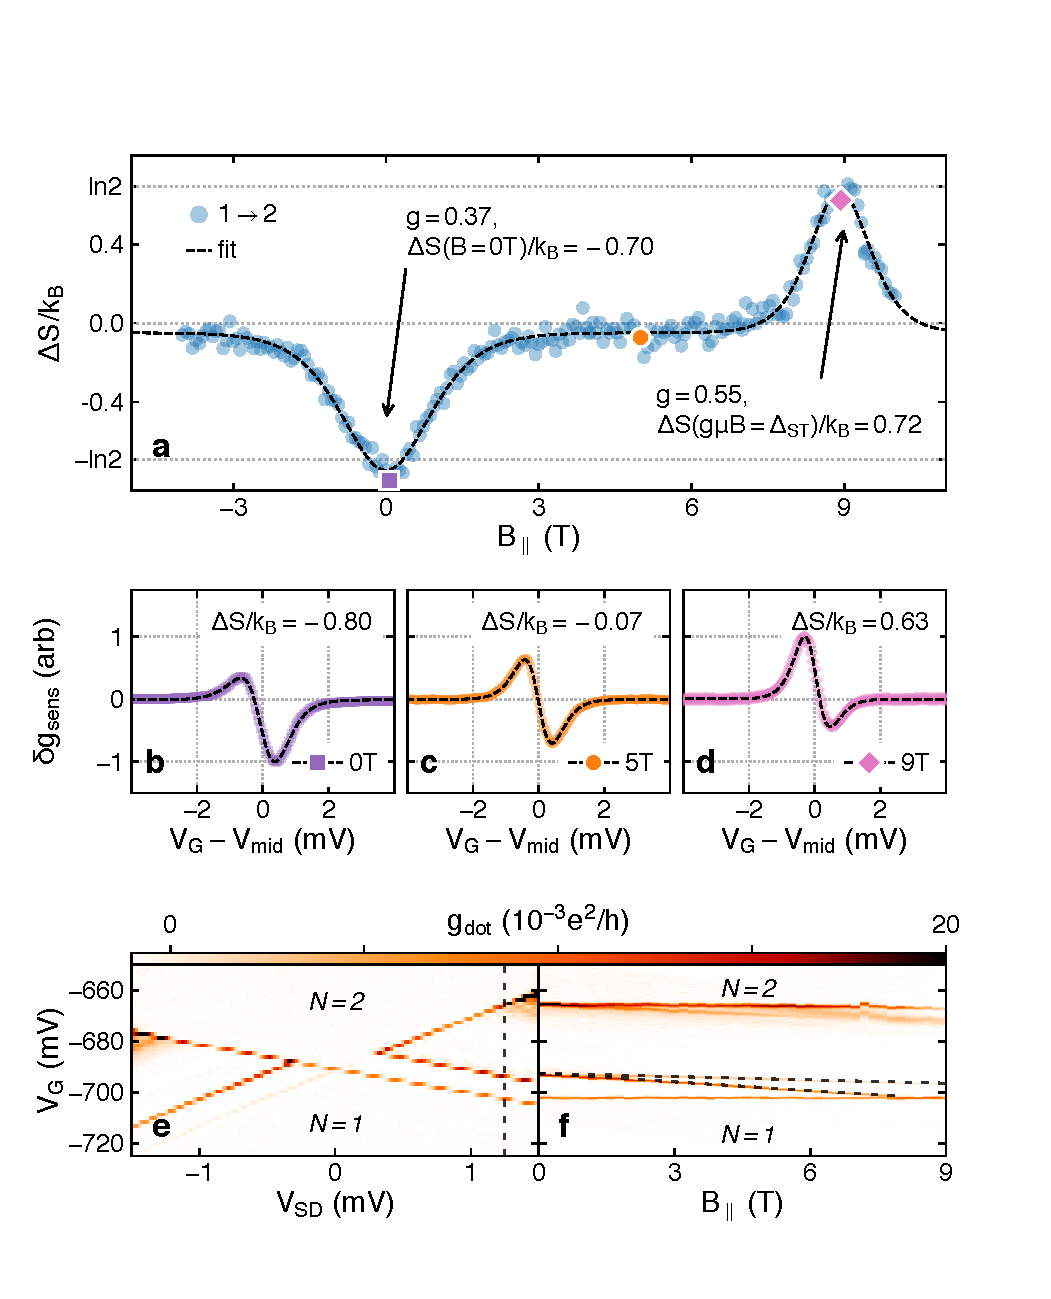
\includegraphics[width=1.0\columnwidth]{../figures/figure_4.pdf}
        \caption{\label{fig:fig4}(a) (a) Transport data through the quantum dot showing the $N=1 \rightarrow 2$ transition. Singlet-triplet splitting is roughly \SI{300}{\micro\electronvolt} and depends on applied field. Dashed line shows where data in (b) are taken. (b) TFixed bias transport data ($V_{SD}$ = \SI{1250}{\micro\electronvolt}). The triplet level is split into T$_+$, T$_0$, and $T_{-}$ (not visible). At \SI[input-protect-tokens]{\sim 9}{\tesla} T$_+$ becomes degenerate with S. g-factor is determined using $T_0$ and $T_+$ fits. (c) Change in entropy, extracted from $dg$ fits, as a function of parallel field. As the field goes from 0 to 10T, entropy of the 2-electron state goes from $0  \rightarrow \ln{2}$, while the entropy of the 1-electron state goes from $\ln{2} \rightarrow 0$. (d), (e), and (f) show characteristic $dg$ traces from which the data in (c) was extracted.}
\end{figure}

The low field (\SI{<5}{\tesla}) results in Fig. \ref{fig:fig4}c can be understood as simply the inverse of Fig \ref{fig:fig3}c. The entropy of the 2-electron ground state remains $0$, in the spin-singlet state, and the entropy of the 1-electron ground state goes from $k_B\ln{2}$ to $0$ due to the Zeeman splitting seen in Fig. \ref{fig:fig3}b. At high field, the 1-electron ground state remains non-degenerate, while the 2-electron ground state picks up a degeneracy of 2 at \SI{9}{\tesla} as the singlet and triplet ($T_+$) levels cross. This confirms that the $dS$ signal can be related directly to a tunable degeneracy in the system. The same splittings in the quantum dot conductance data can be seen in Fig. \ref{fig:fig4}b.

The entropy signal for the 1-2 transition can be fit using Eq. \ref{eqn:p} as the probabilities for the 1-electron groundstates and the following probabilities for the 2-electron singlet-triplet states,
%
\begin{align}
\label{eqn:pst}
        p_{S/T}(B, T) &= \frac{1}{1+ e^{\mp \frac{g\mu_B B - \Delta_{ST}}{k_B T}}}
\end{align}
%
where $\Delta_{ST}$ is the singlet-triplet splitting. Looking at the width of the peaks in $dS$, it is clear that the g-factor changes, along with the singlet-triplet splitting, as the field is increased. Fitting the curve yields $g(B{=}0T)=-0.46$, $g(B{=}9T)=-0.31$, $\Delta_{ST}(B{=}9T)$ = \SI{240}{\micro\electronvolt}, $dS(B{=}0T) = 1.04\ln{2}$, and $dS(B{=}9T) = 1.01\ln{2}$. Each of these values is consistent with the dot transport data and the fits in Fig. \ref{fig:fig3}c.

The results presented in this work have confirmed the degeneracy of the few-electron ground states states, as calculated using only the spin degree of freedom. Magnetic field dependence of the entropy can be fit using simple spin statistics.  Additionally, a technique has been demonstrated to measure the entropy of few-particle states in mesoscopic devices. Future work may take advantage of this strategy to probe the statistics of non-trival electron and quasiparticle states.

%\acknowledgments
% Everyone I might acknowledge is currently an author. Consider moving someone here.

\bibliography{qdentropy}{}
\bibliographystyle{apsrev4-1}

\end{document}